\section{Odometry results and discussion}
\newcommand{\odomCircleRadius}{0.470}
\newcommand{\odomCircleTurns}{0.952}
\newcommand{\odomCircleYaw}{5.98}
\newcommand{\odomCircleDuration}{15.24}
\newcommand{\odomSpiralRadius}{0.470}
\newcommand{\odomSpiralYaw}{36.79}
\newcommand{\odomSpiralDuration}{90.80}
\newcommand{\odomLineLength}{0.970}
\newcommand{\odomLineDuration}{12.14}
\newcommand{\odomLineYawSpan}{0.0124}
\newcommand{\odomLineYawDegrees}{0.71}

Figure~\ref{fig:odometry} retains all logged poses. For each file, $t=(s-s_0)10^{-9}$~s converts nanosecond stamps to elapsed time. Positions remain in the odometry frame; yaw is unwrapped to remove $2\pi$ representation jumps.

\begin{figure}[H]
\centering
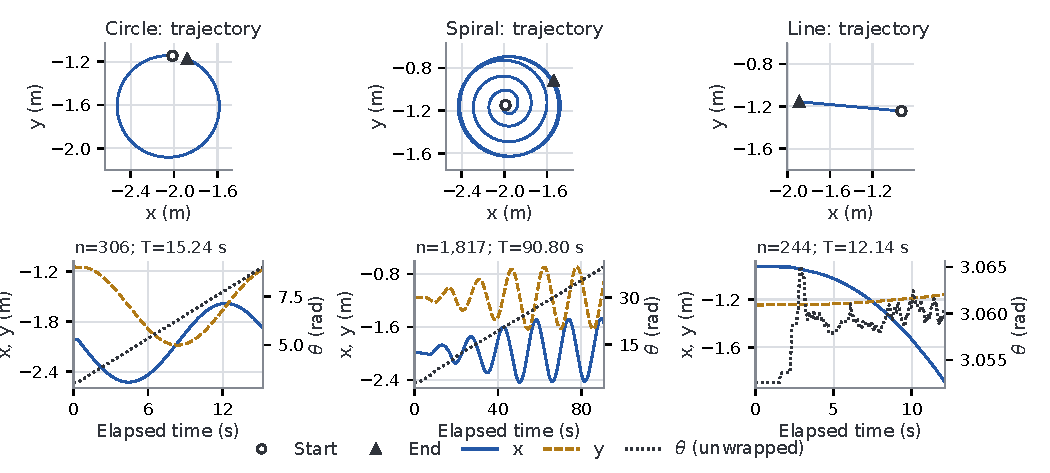
\includegraphics[width=\linewidth]{figures/odometry_results.pdf}
\caption{Odometry: equal-aspect $x$--$y$ paths (top) and position/heading histories (bottom). Left axes show metres; right axes show unwrapped radians. Each run uses its own axis ranges. Titles give sample count $n$ and duration $T$.}
\label{fig:odometry}
\end{figure}

\textbf{Circle:} The resulting radius is \odomCircleRadius~m; $\theta$ increased by \odomCircleYaw~radians during the \odomCircleDuration~s recording. Since this is less than $2\pi$~radians, a full circle was not completed.

\textbf{Spiral:} The outer-loop radius is approximately \odomSpiralRadius~m; $\theta$ increased by \odomSpiralYaw~radians during the \odomSpiralDuration~s recording. The loops initially widen, then overlap near the outer boundary as the radius becomes approximately constant.

\textbf{Line:} The path length is \odomLineLength~m over \odomLineDuration~s, with heading variation of only \odomLineYawSpan~rad (\odomLineYawDegrees$^\circ$). The increasing magnitude of the position slope indicates acceleration.
